\documentclass{resume}

\usepackage{hyperref}
\usepackage{fontawesome}
\usepackage{wasysym} 
\begin{document}

\fontfamily{ppl}\selectfont

\noindent
\begin{tabularx}{\linewidth}{@{}m{0.8\textwidth} m{0.2\textwidth}@{}}
{
    \Large{Kristof G. Herrmann} \newline
    \small{
        \clink{
            \href{mailto:kristof.herrmann@rwth-aachen.de}{kristof.herrmann@rwth-aachen.de} \textbf{·} 
            {\fontdimen2\font=0.75ex +49 151 2014 2005}
            \textbf{·} 
            {\fontdimen2\font=0.75ex Köln, Germany}
        } 
        \begin{flushleft}
            \footnotesize Hochmotivierter \textbf{Mathematiker und Entwickler} (IoT) mit großem Interesse an komplexen Problemenstellungen. Mehr als 2 Jahre Erfahrung in der Entwicklung von industrieller Software von der Shopfloor-Ebene bis in die Cloud. \textbf{Projektleitung}, Anforderungsanalyse, Planung, Testing und Dokumentation.
        \end{flushleft}
    }
} & 
{
    \hfill
    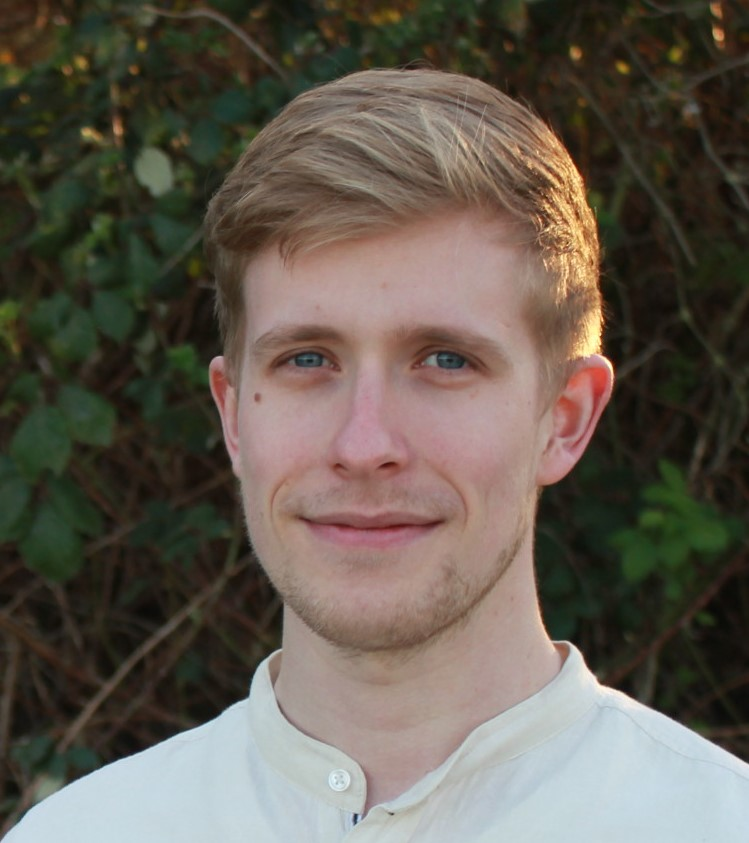
\includegraphics[width=2.7cm]{images/portrait.jpg}
}
\end{tabularx}
\vspace{-5mm}
\begin{center}
\small "Ich möchte meine Fähigkeiten im Projektmanagement weiter verbessern, Verantwortung übernehmen und Teil eines innovativen Teams sein, welches digitale Lösungen mit echten Mehrwerten schafft."
%\vspace{5mm}

%Softwareentwickler für Int Anwendungen mit acht Jahren Erfahrung in der Entwicklung einer breiten Palette von Tools für iOS und Android für eine Reihe von Kunden. 
%Ich habe ausgewiesene Expertise in der Entwicklung von datenmanagement Applikationen. 
%Ich verstehe den Lebenszyklus von Backendsoftware sehr gut und bin sehr fähig in allen Aspekten der Entwicklung, von der Projektplanung über die Anforderungserfassung bis hin zum Schreiben und Testen von Code, Erstellen von Dokumentation. 
%Ich bin derzeit auf der Suche nach einer langfristigen Position, die es mir ermöglicht, meine Fähigkeiten im Projektmanagement weiter zu verbessern.

\vspace{5mm} 
\begin{tabularx}{\linewidth}{@{}*{2}{X}@{}}
% left side %
{
    \csection{ERFAHRUNG}{\small
        \begin{itemize}
            % item 1 %
            \item \frcontent{Senseering GmbH}{Full Stack Software Engineer - Köln}{
            Entwickler einer dezentralen data sharing platform im Sinne von \href{https://www.bmwi.de/Redaktion/DE/Dossier/gaia-x.html}{GAIA-X}. Technischer Berater IoT Lösungen.}{seit April 2020}
             \item \frcontent{WZL der RWTH Aachen}{Werkstudent - Aachen}{Entwickler einer dezentralen data sharing platform im Sinne von \href{https://www.bmwi.de/Redaktion/DE/Dossier/gaia-x.html}{GAIA-X}}{April 2019 - April 2020}
            \item \frcontent{PricewaterhouseCoopers GmbH}{Praktikant Business Intelligence - Düsseldorf}{Entwicklung eines Planungstools für die Wartung und Instandhaltung der Fahrzeuge eines großen, deutschen Transportdienstleisters.}{Oktober 2018 - Februar 2019}
            % item 2 %
            \item \frcontent{RWTH Aachen}{Tutor für höhere Mathematik- Aachen}{}{Oktober 2015 - September 2018}
        \end{itemize}
    }
    \csection{AUSBILDUNG}{\small
        \begin{itemize}
            % item 1 %
            \item \frcontent{M.Sc. Mathematik \footnotesize $\diameter$1.0}{Rheinisch-Westfälische Technische Hochschule Aachen}{}{Herbst 2017- Herbst 2019}
            \item \frcontent{B.Sc. Mathematik \footnotesize $\diameter$1.8}{Rheinisch-Westfälische Technische Hochschule Aachen}{}{Herbst 2014- Herbst 2017}
        \end{itemize}
    }
    \csection{AUSZEICHNUNGEN}{\small
        \begin{itemize}
            % item 1 %
            \item \frcontent{\href{https://www.spaicer.de/}{Springorum-Denkmünze} }{proRWTH - Freunde und Förderer der RWTH Aachen}{}{2020}
        \end{itemize}
    }
} 
% end left side %
& 
% right side %
{
    \csection{SKILLS}{\small
        \begin{itemize}
             \item \textbf{Programmiersprachen \& Datenbanken} \newline
            {\footnotesize Nodejs, Vue, Python, MySQL, Mongodb, Iinfluxdb, Elasticsearch, Redis}
            \item \textbf{Cloud \& Technologien} \newline
            {\footnotesize S3/Azure Blob Storage, EC2, CodeBuild, CodePipeline, CDN, ECS, Azure IoT Hub, Grafana, docker, Portainer, Node Red, Github Actions, DynamoDB, AWS Cognito, KeyCloak, Auth0, IOTA, Nginx, httpd}
            \item \textbf{Mathematik} \newline
            {\footnotesize Partielle Differentialgleichungen \& Maßtheorie, Finanzmathematik, Numerische Analysis}
              \item \textbf{Sprachen} \newline
            {\footnotesize Deutsch, Englisch}
        \end{itemize}
    }
    \csection{PROJEKTE}{\small
        \begin{itemize}
            \item \frcontent{spaicer \clink{\href{https://www.spaicer.de/}{[spaicer.de]}}}{Skalierbare adaptive Produktionssysteme durch KI-Basierte Resilienzoptimierung - Projektverantwortung }{}{Projektverantwortung, IoT, Machine Learning, KI}
            \item \frcontent{obsidian \clink{\href{https://github.com/Senseering/obsidian}{[Senseering/obsidian]}}}{A Nodejs based immutability layer for (industrial) data}{Release pending}{Nodejs, IOTA}
             \item \frcontent{MyDataEconomy \clink{\href{https://www.mydataeconomy.com}{[mydataeconomy.com]}}}{Decentralized IoT data sharing platform for sovereign data exchange.}{}{GAIA-X, Nodejs, Docker, IOTA, InfluxDB}
             \item \frcontent{Duck \clink{\href{https://arzelaascoii.github.io/UAVDocs}{[arzelaascoii.github.io/UAVDocs]}}}{Autonomous flying solar plane built from scratch.}{}{UAV, Ardupilot, ROS, Docusaurus}
        \end{itemize}
    }
    %\csection{OTHER HIGHLIGHTS}{\small
    %%    \begin{itemize}
     %       \item {\footnotesize Gave talk on \textit{Achieving Rapid Response Times in Large Online Services} at Berkeley AMPLab Cloud.}
     %       \item {\footnotesize Led several teams across infrastructure, founded \textit{Google Brain} and was involved in hiring process.}
     %   \end{itemize}
    %}
    %\csection{HOBBIES \& INTERESTS}{\small
    %    \vspace{0.32cm}
    %    \begin{tabularx}{\linewidth}{@{}*{4}{>{\centering\arraybackslash}X}@{}}
    %%        {\centering
     %       
\includegraphics[width=0.8cm]{images/userexperience.png}
     %%       } &
       %     {\centering
        %    
\includegraphics[width=0.8cm]{images/lamp.png}
         %   } & 
         %   {\centering
        %    
\includegraphics[width=0.8cm]{images/healthcare.png}
    %        } &
     %       {\centering
     %       
\includegraphics[width=0.8cm]{images/cauldron.png}
     %       } \\
     %       {\footnotesize UI/UX} & {\footnotesize Problem Solving} & {\footnotesize Healthcare} & %{\footnotesize Open Source}
     %   \end{tabularx}
    %}
}
\end{tabularx}
\end{center}

\begin{center}

\begin{tabularx}{\linewidth}{@{}*{3}{X}@{}}
\centering{\href{https://www.linkedin.com/in/kgherr}{ \Large  \faLinkedinSquare } }
&
\centering{ \href{https://github.com/ArzelaAscoIi}{\Large \faGithub } }
&{\hspace{25mm}\href{https://www.medium.com/@Kristof.herrmann}{\Large \faMedium }}
\\
\centering\small kgherr &
\centering\small ArzelaAscoIi  & 
\centering\small @Kristof.herrmann
\end{tabularx}

\end{center}
\end{document}